%\vskip -27.7pt
\begin{IEEEbiography}
[{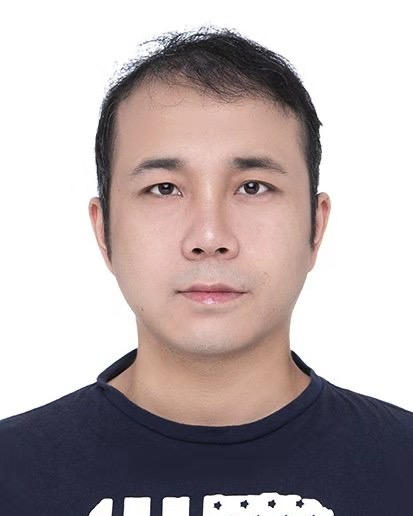
\includegraphics[width=1in,height=1.25in,clip,keepaspectratio]{./photos/Chunfeng_Liu}}] 
{Chunfeng Liu} 
received the bachelor degree in automation from Tsinghua University, Beijing,
China, in 2009 and the master degree in microelectronics from Tsinghua
University, Beijing, China, in 2015. He is currently a PhD student with the Chair
of Electronic Design Automation, Technical University of Munich (TUM). His research interests focus on
computer-aided design for microfluidic biochips. 
\end{IEEEbiography}
\vskip -27.7pt
\begin{IEEEbiography}
[{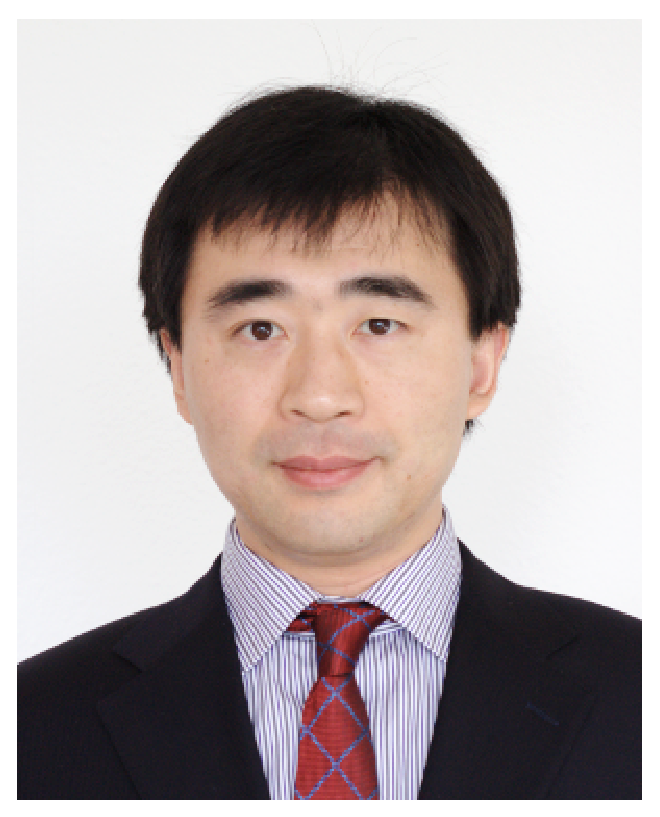
\includegraphics[width=1in,height=1.25in,clip,keepaspectratio]{./photos/Bing_Li}}] 
{Bing Li} 
received the Dr.-Ing. degree from 
Technical University of Munich (TUM), Munich, Germany, in
2010 and finished the Habilitation there in 2018. He
is currently a researcher with the Chair of Electronic
Design Automation, TUM. His current research interests include high-performance and lower-power
design, design automation for microfluidic biochips,
as well as emerging systems. He has served on
the Technical Program Committees of several conferences including ICCAD, DATE,
ASP-DAC, etc.
\end{IEEEbiography}
\vskip -27.7pt
\begin{IEEEbiography}
[{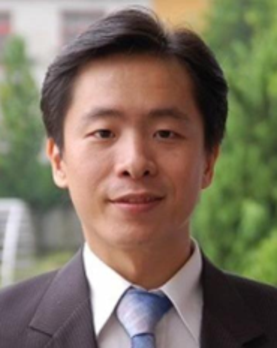
\includegraphics[width=1in,height=1.25in,clip,keepaspectratio]{./photos/Tsungyi}}] 
{Tsung-Yi Ho} (M'08--SM'12) received his Ph.D. degree in Electrical Engineering from National Taiwan
University, Taipei, Taiwan, in 2005.  He is a Professor with the Department of Computer 
Science of National Tsing Hua University, Hsinchu, Taiwan. His research interests include 
design automation and test for microfluidic biochips and nanometer integrated circuits.
Dr. Ho was a recipient of the Best Paper Awards at the VLSI Test Symposium (VTS) in 2013 and IEEE
TCAD in 2015. Currently he serves as an ACM Distinguished Speaker, 
a Distinguished Lecturer of the IEEE Circuits and
Systems Society, and Associate Editor of the ACM JETC, ACM TODAES,
ACM TECS, and IEEE TVLSI, and the Technical Program Committees of
major conferences, including DAC, ICCAD, DATE, ASP-DAC, ISPD, etc.
\end{IEEEbiography}
\vskip -27.7pt
\begin{IEEEbiography}
[{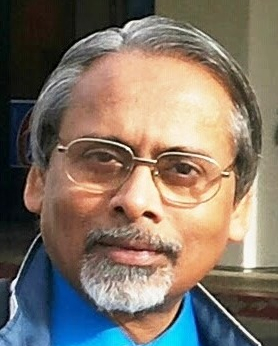
\includegraphics[width=1in,height=1.25in,clip,keepaspectratio]{./photos/BBB_TCAD_Photo}}]
{Bhargab B. Bhattacharya} (F'07) is currently serving as Distinguished Visiting
Professor of Computer Science \& Engineering at the Indian Institute of
Technology Kharagpur. Prior to that, he had been on the faculty of the Indian
Statistical Institute, Kolkata, for over 35 years. His research interest
includes digital logic testing, and electronic design automation for integrated
circuits and microfluidic biochips. He has published more that 400 technical
papers and he holds ten US Patents. He is a Fellow of the Indian National
Academy of Engineering and a Fellow of the National Academy of Sciences
(India).
\end{IEEEbiography}
\vskip -27.7pt
\begin{IEEEbiography}
[{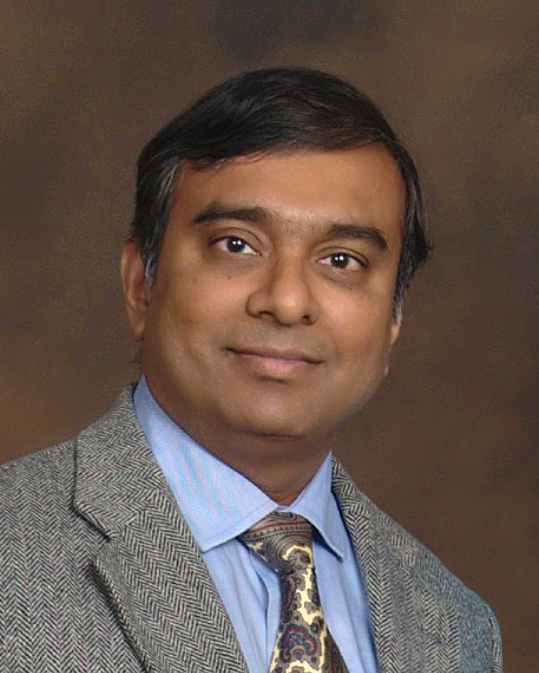
\includegraphics[width=1in,height=1.25in,clip,keepaspectratio]{./photos/Chakrabarty_Krishnendu}}]
{Krishnendu Chakrabarty} (F'08) received the Ph.D. degree from the University of Michigan, Ann Arbor, in 1995. He is now the John Cocke Distinguished Professor and Department Chair of Electrical and Computer Engineering at Duke University. His current research projects include: testing, design-for-testability, and fault diagnosis of 3D SOCs and AI/ML hardware; microfluidic biochips; hardware security. Prof. Chakrabarty is a Fellow of ACM, a Fellow of IEEE, a Fellow of AAAS, and a Golden Core Member of the IEEE Computer Society. 
\end{IEEEbiography}
\vskip -27.7pt
\begin{IEEEbiography}
[{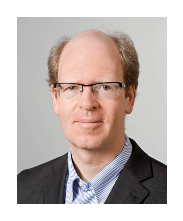
\includegraphics[width=1in,height=1.25in,clip,keepaspectratio]{./photos/Ulf_Schlichtmann}}] 
{Ulf Schlichtmann} (S'88--M'90--SM'18) received the Dipl.-Ing. and Dr.-Ing.
degrees in electrical engineering and information technology from Technical
University  of  Munich (TUM), Munich, Germany, in 1990 and 1995,  respectively.

He is Professor and the Head of the Chair of Electronic Design Automation at
TUM. He joined TUM in 2003, following 10 years in industry. His current
research interests include computer-aided design of electronic circuits and
systems, with an emphasis on designing reliable and robust systems.
Increasingly, he focuses on emerging technologies such as lab-on-chip and
photonics.
\end{IEEEbiography}

\vfill

